\section{Approach}

With the language to implement introduced, we proceed with presenting our approach.

\subsection{Architecture}
\label{sec:architecture}

\begin{figure}
  \centering
  \begin{tikzpicture}
    \umlclass[template={T}, x=0, y=0, anchor=north west]{BrainfuqInterpreter}{}{
      $+$ interpret\_program(p: \texttt{str}): \texttt{tuple[T, dict[int, np.uint8]]} \\
    }

    \umlclass[type=abstract, template={T}, x=16.8, y=0, anchor=north east]{BrainfuqQuantumInterpreter}{
      $\#$ quantum\_ptr : \texttt{int} \\
      $\#$ qubit\_map : \texttt{dict[int, int]} \\
      $\#$ control\_qubit\_ptr : \texttt{int | None} \\
      $-$ measurement\_control\_active : \texttt{bool} \\
      $-$ next\_idx : \texttt{int}
    }{
      $+$ apply\_operation(op : str) : \texttt{None} \\
      \umlvirt{$+$ return\_state() : T} \\
      \umlvirt{$\#$ apply\_x() : \texttt{None}} \\
      \umlvirt{$\#$ measure() : \texttt{None}} \\
      $-$ move\_right() : \texttt{None} \\
      $-$ move\_left() : \texttt{None} \\
    }

    \umlclass[x=0, y=-3.2, anchor=north west]{BrainfuqClassicalInterpreter}{
      $-$ classical\_tape : \texttt{dict[int, np.uint8]} \\
      $-$ classical\_ptr : \texttt{int} \\
    }{
      $+$ apply\_operation(op : \texttt{str}): \texttt{int} \\
      $+$ return\_state(): \texttt{dict[int, np.uint8]} \\
    }

    \umlclass[x=0, y=-9.5, anchor=south west]{BrainfuqSimulator}{
      $-$ quantum\_tape: \texttt{dict[int, complex]} \\
    }{
      $+$ return\_state() : \texttt{tuple[dict[int, complex], dict[int, int]]} \\
      $\#$ apply\_x() : \texttt{None} \\
      $\#$ measure() : \texttt{None} \\
    }

    \umlclass[x=16.8, y=-9.5, anchor=south east]{QiskitBrainfuqInterpreter}{
      $+$ operations: \texttt{list[tuple]} \\
    }{
      $+$ return\_state() : QuantumCircuit \\
      $\#$ apply\_x() : \texttt{None} \\
      $\#$ measure() : \texttt{None} \\
    }

    % Generalization / Inheritance Relationship
    \umlVHVinherit[arm2=-3.4cm, stereo={T $\to$ tuple[dict[int, complex], dict[int, int]]}]{BrainfuqSimulator}{BrainfuqQuantumInterpreter}
    \umlVHVinherit[arm2=-3.4cm, stereo={T $\to$ QuantumCircuit}]{QiskitBrainfuqInterpreter}{BrainfuqQuantumInterpreter}
    \umlVHVcompo[arm2=0.5cm, arg=classical\_interpreter, pos=0.45, mult=1]{BrainfuqInterpreter}{BrainfuqClassicalInterpreter}
    \umlVHcompo[arm1=-0.9cm, arg=quantum\_interpreter, mult=1, align=right, pos=1.48, anchor2=5]{BrainfuqInterpreter}{BrainfuqQuantumInterpreter}
  \end{tikzpicture}
  \caption{\textsc{Uml} diagram of our \textsc{Brainfuq} interpreter. Some attributes and methods, including those related to $H$ and $T$ gates, were omitted to improve clarity. To improve the readability of attribute and method names, leading underscores are omitted.}
  \label{fig:uml}
\end{figure}

Our goal was to design a modular architecture that strikes a good balance between clearly separating concerns and limiting redundancy. The resulting class structure is depicted in the \textsc{uml} diagram depicted in \cref{fig:uml}. We briefly go through each component.
\begin{description}
  \item[\texttt{BrainfuqInterpreter}] This is the top-level component responsible for parsing \hb{} programs. Its main concern is stepping through the program and delegating each command to be executed either to the classical or to the quantum interpreter. When the end of the program is reached, the \texttt{return\_state()} methods of the classical and quantum interpreters are called to report the final state.
  \item[\texttt{BrainfuqClassicalInterpreter}] This component maintains the classical tape, and reports possible jumps to \texttt{BrainfuqInterpreter}.
  \item[\texttt{BrainfuqQuantumInterpreter}] The second attribute of \texttt{BrainfuqInterpreter} handles quantum operations. In our case, there are two possible quantum-computing-related problems to solve: simulating the program and converting it into a \qiskit{} circuit. \texttt{BrainfuqQuantumInterpreter} is an abstract class handling the greatest common denominator of those tasks: It maintains the quantum pointer together with the layout of the qubit tape, and stores if the next gate is controlled, which qubit that gate is controlled on, and if the qubit should be applied at all based on the last measurement.
  \item[\texttt{BrainfuqSimulator}] The first class inheriting from \texttt{BrainfuqQuantumInterpreter} handles the simulator logic. We refer to \cref{sec:approach-quantum-tape} for more details about how this class handles simulation together with its base class.
  \item[\texttt{QiskitBrainfuqInterpreter}] The other class inheriting from \texttt{BrainfuqQuantumInterpreter} builds a \qiskit{} circuit from the given instructions. We provide further details in \cref{sec:approach-translations}.
\end{description}

% This should be the most detailed section in general. How did you approach to solve your problem? What worked and what did not work. Here, you should also add your evaluations.

\subsection{Simulation}
\label{sec:approach-quantum-tape}

The main challenge in implementing a \hb{} simulator is the representation of the quantum tape.
In classical \bfck{} the tape can be implemented as a plain hash map from indices to tape values.
The indices are signed integers, i.e., they can take on positive and negative values as the pointer is moved left and right.
The tape values are typically bytes representing an 8-bit unsigned integer.

In our implementation, we attempt to apply this approach to the quantum tape, which requires some creativity to accommodate the properties of quantum states.
While a naive map from indices to single qubits seems straightforward, it is not sufficient, as it can only be used to store product states.
As the gates of the \hb{} specification form a universal basis for quantum gates, arbitrary, and in particular entangled, quantum states can be computed.
To represent arbitrary quantum states, we transition to a map $\qtape$ from basis states to complex amplitudes.
Although such a map is capable of storing arbitrary states similar to a plain state vector, the representation of the basis states remains a challenge.
Given that the quantum tape is infinite, i.e., the indices run from $-\infty$ to $\infty$, there are no boundaries that define a reference frame for specifying basis states.
Instead, we introduce a $\qmap$ that maps from the indices on the quantum tape to progressively positive qubit indices.
The idea is that when we move the quantum pointer to a new location, it is always added on the same side in our classical representation of the quantum state.
The initial state of our system is $\qtape = \{0: 1.0\}$ and $\qmap = \{0: 0\}$.
When we move the pointer to the left, the  $\qmap$ is extended to ${0: 0, -1: 1}$, or analogously to ${0: 0, 1: 1}$ if we move it right to index 1 on the tape.
Note, that the $\qtape$ remains $\{0: 1.0\}$ for now.
This is because we add new qubits as the most significant bit position, i.e., as $q_n$ in $\ket{q_n ... q_0}$.
For optimization purposes, we generally omit the leading zeros in the bitstrings representing the basis states, such that the $\qtape$ does not change when we move the pointer to an unseen index.
As a further optimization, we only store those amplitudes in the $\qtape$ map that are not zero.
Apart from incorporating the qubit mapping, applying gates and measuring qubits work equivalently as in standard statevector simulators.

For readers interested in a standalone implementation of the simulator that does not use the surrounding architecture, we refer to \texttt{brainfuq\_interpreter/brainfuq\_interpreter\_old.py}.

\subsection{Translation to \qiskit{}}
\label{sec:approach-translations}

Implementing the translator to \qiskit{} is comparatively straightforward, but it still provides a few challenges. The first one was to ensure that the qubits in the resulting \qiskit{} circuit follow the same order as the ones on the quantum tape. With this, an on-the-fly construction of the circuit is out of question. To accommodate this, we store all operations to apply with their target index, potential quantum control index, and potential classical control index in the list \texttt{operations}. In \texttt{return\_state()}, where we know all existing qubits, we finally construct the \qiskit{} circuit.
Another challenge was determining how the \texttt{?} operation should be handled. In our implementation, we write each measurement to a new classical bit of the \qiskit{} circuit, and then implement \texttt{?} using the \texttt{if\_test()} method of \qiskit{} circuits applied to the last used classical bit.
We note that, to facilitate the creation of \bfck{} programs, we also implemented a rudimentary translator for the reverse direction.

\subsection{Examples}
\label{sec:approach-examples}

To showcase the functionality of our interpreter and translators, we implemented small instances of some quantum algorithms in the \texttt{examples} folder of the repository.
The script \texttt{examples/ghz.py} (s. Listing \ref{lst:ghz_example}) initializes a $N$-qubit GHZ state.
After applying the Hadamard gate on the first qubit, it leverages classical instructions to iteratively add CNOT gates and move the quantum pointer.
The number of qubits of the resulting state is controlled by the parameter variable $N$, which is used to set up the loop counter variable that is decremented at the end of each iteration.
For instance $N=5$ produces the \hb{} program \texttt{\textasciitilde +++++[\#\}*-]}.
As expected, processing the string puts the quantum tape into the state $\frac{1}{\sqrt{2}} (\ket{00000} + \ket{11111})$, which we confirm by printing the string representation of our quantum simulator.

Further, \texttt{examples/quantum-teleportation.py} implements the circuit for teleporting a qubit through a shared pair of entangled qubits.
In addition to the standard quantum logic, it also uses the \texttt{?} instruction to apply Z and X gates based on the classical measurement results.
We initialize q0 as $\ket{-}$ through \texttt{\textasciitilde ;;;}, i.e., a Hadamard and 4 consecutive T gates, simulating a Z gate.
We confirm that after the teleportation logic, the state of the system features q0 and q1 in their collapsed measurement state and q2 in the $\ket{-}$ state.
Printing the entire system state, we get the \texttt{-0.707 |011⟩ + 0.707 |010⟩} or versions with arbitrary other combinations of the first two qubits.

Lastly, \texttt{examples/grover.py} shows how different software components work together.
To start, it translates a \qiskit{} Grover operator, obtained by concatenating a phase oracle and a diffusion operator, into a \hb{} program string.
This string is then embedded into the full \hb{} program as the body to a loop which is executed for the optimal number of Grover iterations which we calculate classically for the given oracle.
We prefix the program with Hadamard gates, setting the search qubits into an equal superposition and an optional suffix for measuring the search qubits.
In the script, we use an oracle which marks exactly the basis state consisting only of 1-bits, i.e., only one solution.
To prevent this oracle from blowing up in terms of the number of used basis gates, we implement a version with $N-2$ auxiliary qubits.
Although this oracle is relatively compact, it still produces \hb{} programs with a significant count of overall instructions.
For $N=6$, for instance, the \hb{} program of a single Grover operator is comprised of 21255 classical instructions (including pointer shifts), which results in an overall runtime of almost $30s$.
Running the script with \texttt{measure=False} and $N=3$ produces the following state where the last qubit is an auxiliary: \texttt{0.972 |1110⟩ - 0.088 |1100⟩ - 0.088 |1000⟩ - 0.088 |0000⟩ - 0.088 |0100⟩ - 0.088 |1010⟩ - 0.088 |0010⟩ - 0.088 |0110⟩}.

\subsection{Edge Case Inputs}
\label{sec:approach-edge-cases}

Given the \hb{} instructions presented in \Cref{sec:background}, there are some edge case inputs for which the expected behavior of the system is unclear.
For repeated \texttt{\#} without a resetting gate instruction, i.e. \texttt{*}, \texttt{\textasciitilde} or \texttt{;} in between, the last \texttt{\#} governs which qubit controls the next gate.
If the program does not feature any measurement instructions \texttt{:} before a \texttt{?}, the next gate is not executed as the last measurement did not exist and hence was not $1$ in particular.
